%! Author = pierre
%! Date = 16/04/2024

\documentclass[10pt]{article}

\usepackage[utf8]{inputenc}
\usepackage{amsmath}
\usepackage{amsfonts}
\usepackage{amssymb}
\usepackage{graphicx}
\usepackage{hyperref}
\usepackage{natbib}
\usepackage{geometry}
\usepackage{tikz}
\usepackage{pgfplots}
\usepackage{subcaption}
\usepackage{comment}
\usepackage{tabularx}
\usepackage{helvet}
\usepackage{float}
\renewcommand{\familydefault}{\sfdefault}
\pgfplotsset{compat=1.17}

\geometry{a4paper, margin=1in}

\hypersetup{
    colorlinks=true,
    linkcolor=blue,
    urlcolor=black,
    citecolor=blue,
}

\title{State of the Art: Graph Neural Networks}
\author{Pierre LAPOLLA}
\date{\today}


\begin{document}

    \maketitle
    \tableofcontents

    \newpage
    \begin{abstract}
        Our goal is to develop a model for predicting optimal itineraries based on selectable criteria, which may include minimal carbon footprint, health considerations, and potentially a combination of these factors.
        The criteria selection is a difficult task as we want relevant ones and ones that are available in public datasets as we will not collect any new data here.
        Some criteria that we could consider are: minimal carbon footprint, air quality exposure, physical activity.
        We want our solution to add something new to the existing solutions: balancing multiple criteria and maybe allows weighting them.
        Graph neural networks (GNNs) are a promising approach for this problem, as they can be dynamic.
        If we manage to produce a solution to this problem, it could be used in various applications, such as enhancing existing apps to offer more personalized routing options.
        However we expect some challenges and limitations, such as data availability, computational complexity, and the need for real-time processing.
    \end{abstract}


    \section{Key algorithms and Methods}\label{sec:key-algorithms-and-methods}
    Pathfinding algorithm are widely used in various applications, network routing, video games, etc.
    Below is a comparison table of some of the most popular algorithms:

    \begin{table}[h]
        \centering
        \begin{tabularx}{\textwidth}{|X|X|X|X|X|}
            \hline
            \textbf{Algorithm} & \textbf{Best for}                                  & \textbf{Time Complexity}          & \textbf{Space Complexity} & \textbf{Negative Weights?} \\ \hline
            Dijkstra’s         & Shortest paths from a single source in a graph     & \(O(V^2)\) or \(O(E + V \log V)\) & \(O(V)\)                  & No                         \\ \hline
            A*                 & Pathfinding with heuristics to speed up the search & \(O(E)\)                          & \(O(V)\)                  & No                         \\ \hline
            Bellman-Ford       & Graphs with negative weight edges                  & \(O(VE)\)                         & \(O(V)\)                  & Yes                        \\ \hline
            Floyd-Warshall     & Shortest paths between all pairs of nodes          & \(O(V^3)\)                        & \(O(V^2)\)                & Yes                        \\ \hline
        \end{tabularx}
        \caption{Comparison of Route Optimization Algorithms}
        \label{tab:route_optimization_algorithms}
    \end{table}


    \section{Multi-Objective Optimization}\label{subsec:multi-objective-optimization}
    The key algorithms and methods are not sufficient to solve our problem.
    These algorithms can optimize multiple criteria simultaneously, which is very close to what we want.

    \subsection{Genetic Algorithms}\label{subsec:genetic-algorithms}
    These algorithms mimic natural selection, with crossovers and mutations.
    They are good for finding the global optimum of a function.
    However, they are not good for real-time applications.

    \subsection{Pareto Optimization}\label{subsec:pareto-optimization}
    Pareto optimization is a multi-objective optimization technique that aims to find the best trade-offs between multiple objectives.
    It is based on the Pareto principle, which states that for any given problem, some solutions are better than others.
    This solution is good for our problem as we want to balance multiple criteria.
    However it is not dynamic, which is a limitation.


    \section{Graph Neural Networks}\label{sec:graph-neural-networks}
    Despite their efficiency, the multi-objective optimization algorithms are not good options for us.
    We want scalable and dynamic solutions, which is why we are considering Graph Neural Networks (GNNs).
    This section is largely based on the work of~\cite{ref1}.
    It contains lots of references that we can use to deepen our understanding of the topic.

    \subsection{Overview of Graph Neural Networks}\label{subsec:overview-of-graph-neural-networks}
    Graph Neural Networks (GNNs) are a class of deep learning models designed to handle graphs as input data.
    Traditional neural networks assume that the input data is in a Euclidean space, which is not the case for graphs.
    They also treat inputs as independent of each other, which is not true for graph data.
    These differences allows GNNs to capture the structure of the graph and the relationships between nodes.
    They are powerfull tools for tasks such as node classification, link prediction, and graph classification.

    \subsection{Types of GNN Architectures}\label{subsec:types-of-gnn-architectures}
    The paper~\cite{ref1} describes four types of GNN architectures where we can classify most other GNNs:

    \begin{itemize}
        \item \textbf{Recurrent Graph Neural Networks (RecGNNs)}: they aim to learn node representations with recurrent architectures.
        They assume nodes are constantly exchanging information with their neighbors.
        \item \textbf{Convolutional Graph Neural Networks (ConvGNNs)}: they generalize the convolution from euclidean space to graph data.
        The idea is to aggregate information from neighbors to update the node representation.
        \item \textbf{Graph Autoencoders (GAEs)}: they aim to learn a low-dimensional representation of the graph.
        They can reconstruct the graph from this representation.
        \item \textbf{Spatial-Temporal Graph Neural Networks (STGNNs)}: they are designed for spatio-temporal data.
        They can learn hidden patterns from spatial and temporal data.
    \end{itemize}

    \begin{table}[h]
        \centering
        \begin{tabularx}{\textwidth}{|X|X|X|X|X|}
            \hline
            \textbf{Feature}     & \textbf{RecGNNs}                                                & \textbf{ConvGNNs}                               & \textbf{GAEs}                                               & \textbf{STGNNs}                                \\ \hline
            \textbf{Core Idea}   & Iterative processing of node information to reach stable states      & Generalize convolution operations to graph data   & Encode graph structure into a latent, low-dimensional space   & Integrate both spatial and temporal graph data    \\ \hline
            \textbf{Use Case}    & Complex relational reasoning, dynamic graph updates             & Node classification, community detection          & Graph reconstruction, link prediction                         & Dynamic prediction, traffic forecasting           \\ \hline
            \textbf{Advantages}  & Captures dynamic changes in graph structure                     & Efficient in learning node representations        & Useful in unsupervised learning tasks                         & Handles graphs evolving over time                 \\ \hline
            \textbf{Limitations} & High computational cost for large graphs                        & Limited by local neighborhood information         & Requires large datasets for training                          & Complex model architectures and computations      \\ \hline
        \end{tabularx}
        \caption{Comparison of Graph Neural Network Architectures}
        \label{tab:gnn_comparison}
    \end{table}


    From these architectures, we can assume that STGNNs are the most relevant for our problem as our data will likely be space and time dependent.

    \subsection{Applications}\label{subsec:applications}

    \begin{itemize}
        \item \textbf{Node Classification}: assign a label to each node in the graph.
        \item \textbf{Graph Classification}: assign a label to the entire graph.
        \item \textbf{Link Prediction}: predict the existence of a link between two nodes.
        \item \textbf{Computer Vision}: use GNNs for image segmentation, object detection, etc.
        \item \textbf{Natural Language Processing}: use GNNs for text classification, sentiment analysis, etc.
        \item \textbf{Recommender Systems}: use GNNs to recommend products, movies, etc.
        \item \textbf{Drug Discovery}: use GNNs to predict molecular properties.
        \item \textbf{Traffic Prediction}: use GNNs to predict traffic flow, congestion, etc.
    \end{itemize}

    The paper~\cite{ref1} refers to three other papers that used STGNNs~\cite{ref5,ref6,ref7}~for traffic problems.


    \section{Primary Studies}\label{sec:primary-studies}

    \subsection{First Study}\label{subsec:first-study}
    A Graph Pointer Network-Based Multi-Objective Deep Reinforcement Learning Algorithm for Solving the Travelling Salesman Problem~\cite{ref8}.

    \begin{itemize}
        \item \textbf{Context}:
        This research is based on multi-objective optimization problems and uses the travelling salesman problem as a case study.
        With new methods to process sequential and temporal data, notably qith GNNs, the authors propose a new algorithm to solve the TSP.
        \item \textbf{Problem}:
        The paper addresses the need for more sophisticated algorithms that can effectively manage multiple objectives without sacrificing performance on ny single objective.
        \item \textbf{Data}:
        The authors generated their data using the random generator from PyTorch.
        The training set has 500,000 samples and the validation set has 1,000 samples.
        Note: we could use the same method if we can properly model our problem and the data we need.
        \item \textbf{Results}:
        The authors used a similar comparison test than other paper they cited.
        We can see in the image below that their model (MODGRL) o utperforms the other models.
        \begin{figure}[H]
            \centering
            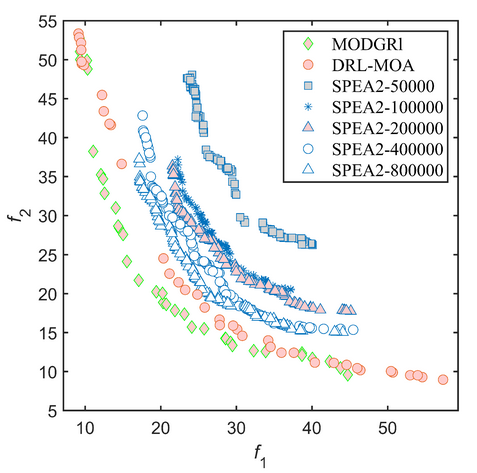
\includegraphics[width=0.5\textwidth]{resources/first_study_results}
            \caption{Comparison of MODGRL with other models}
            \label{fig:modgrl_comparison}
        \end{figure}
        \item \textbf{Future Work}:
        The paper emphasizes the potential for further improvement and application of such models to even more complex and varied multi-objective optimization problems.
        The research suggests that leveraging the advancements in graph neural networks and deep reinforcement learning could lead to significant breakthroughs in various real-world applications requiring multi-objective decision-making.
    \end{itemize}


    \section{Methods Comparison}\label{sec:methods-comparison}
    We will here make a comparison between the methods we have seen so far.


    \section{Gaps and Opportunities}\label{sec:gaps-and-opportunities}
    %Based on your review, identify any gaps in current methodologies or areas where improvements could be made.
    %This could involve combining algorithms, enhancing existing models with real-time data inputs, or applying novel
    %machine learning techniques.


    \section{Conclusion}\label{sec:conclusion}
    %Provide a summary that ties together all your findings, outlining which methods are most promising for your
    %specific objectives and why.


    \section{TODO/Notes}\label{sec:todo/notes}
    travel (time) prediction (eta) on graph nn, chercher avec une contrainte en plus (ex: paratransit), check auteurs, check refs
    theorie des graphes vite fait
    comment predire le temps de trajet avec gnn
    comment etendre cette pred pour ajouter des contraintes
    pas un seul critere parce que google meilleur que nous

    separate graphs: (static structure, static features), (static struture, time-varying features), (time-varying
    structure, static features), (time-varying structure, time-varying features)
    what we will do? first: static structure and static features
    then: static structure and time-varying features

    pas de dataset complet, que des adjacency lists, pas de données supplementaires
    machine learning stanford (cs224w)

    papers with code: papier + database ou code

    chercher papier avce etde primaire (voir pytorch geometric temporal dataset), lister papiers qui font une etude primaire et les comparer
    e qu'il ont en donnees, contexte (ce qu'ils font), la problematique, leur resultats, les perspectives et futurs

    presentation power point avec pdf deja fait, liste du dessus et presentation des bases de données
    but: definir ce qu'on va faire

    %\newpage
    \bibliographystyle{unsrt}
    \bibliography{main}

\end{document}